% CHI keyboard work

\lecture{Application: Touchscreen typing}{Touchscreen}

\begin{frame}
	\frametitle{Typing on touchscreens}
	\begin{itemize}
		\item Most people have smartphones
		\item Most smartphones have touchscreens
		\item Touchscreens are small
		\item Keyboards on touchscreens are small
		\item Typing on them is hard!
		\begin{itemize}
			\item \ldots but people type on them a lot
		\end{itemize}
	\end{itemize}
\end{frame}

\begin{frame}
	\frametitle{Background 1: Why is it hard?}
	\begin{itemize}
		\item Occlusion of target by finger
		\item `fat finger' problem
		\item Small targets
		\item Demo: \url{http://bit.ly/1nBws97}
		\visible<2->{
			\item Quite a bit of work in this area:
			\begin{itemize}
				\item Holz and Baudisch
				\item Henze (100,000,000 taps)
			\end{itemize}
			\item Collecting data is fairly easy
			}
	\end{itemize}
\end{frame}

\begin{frame}
	\frametitle{Background 2: All users are different}
	\begin{figure}[tbh]
		\centering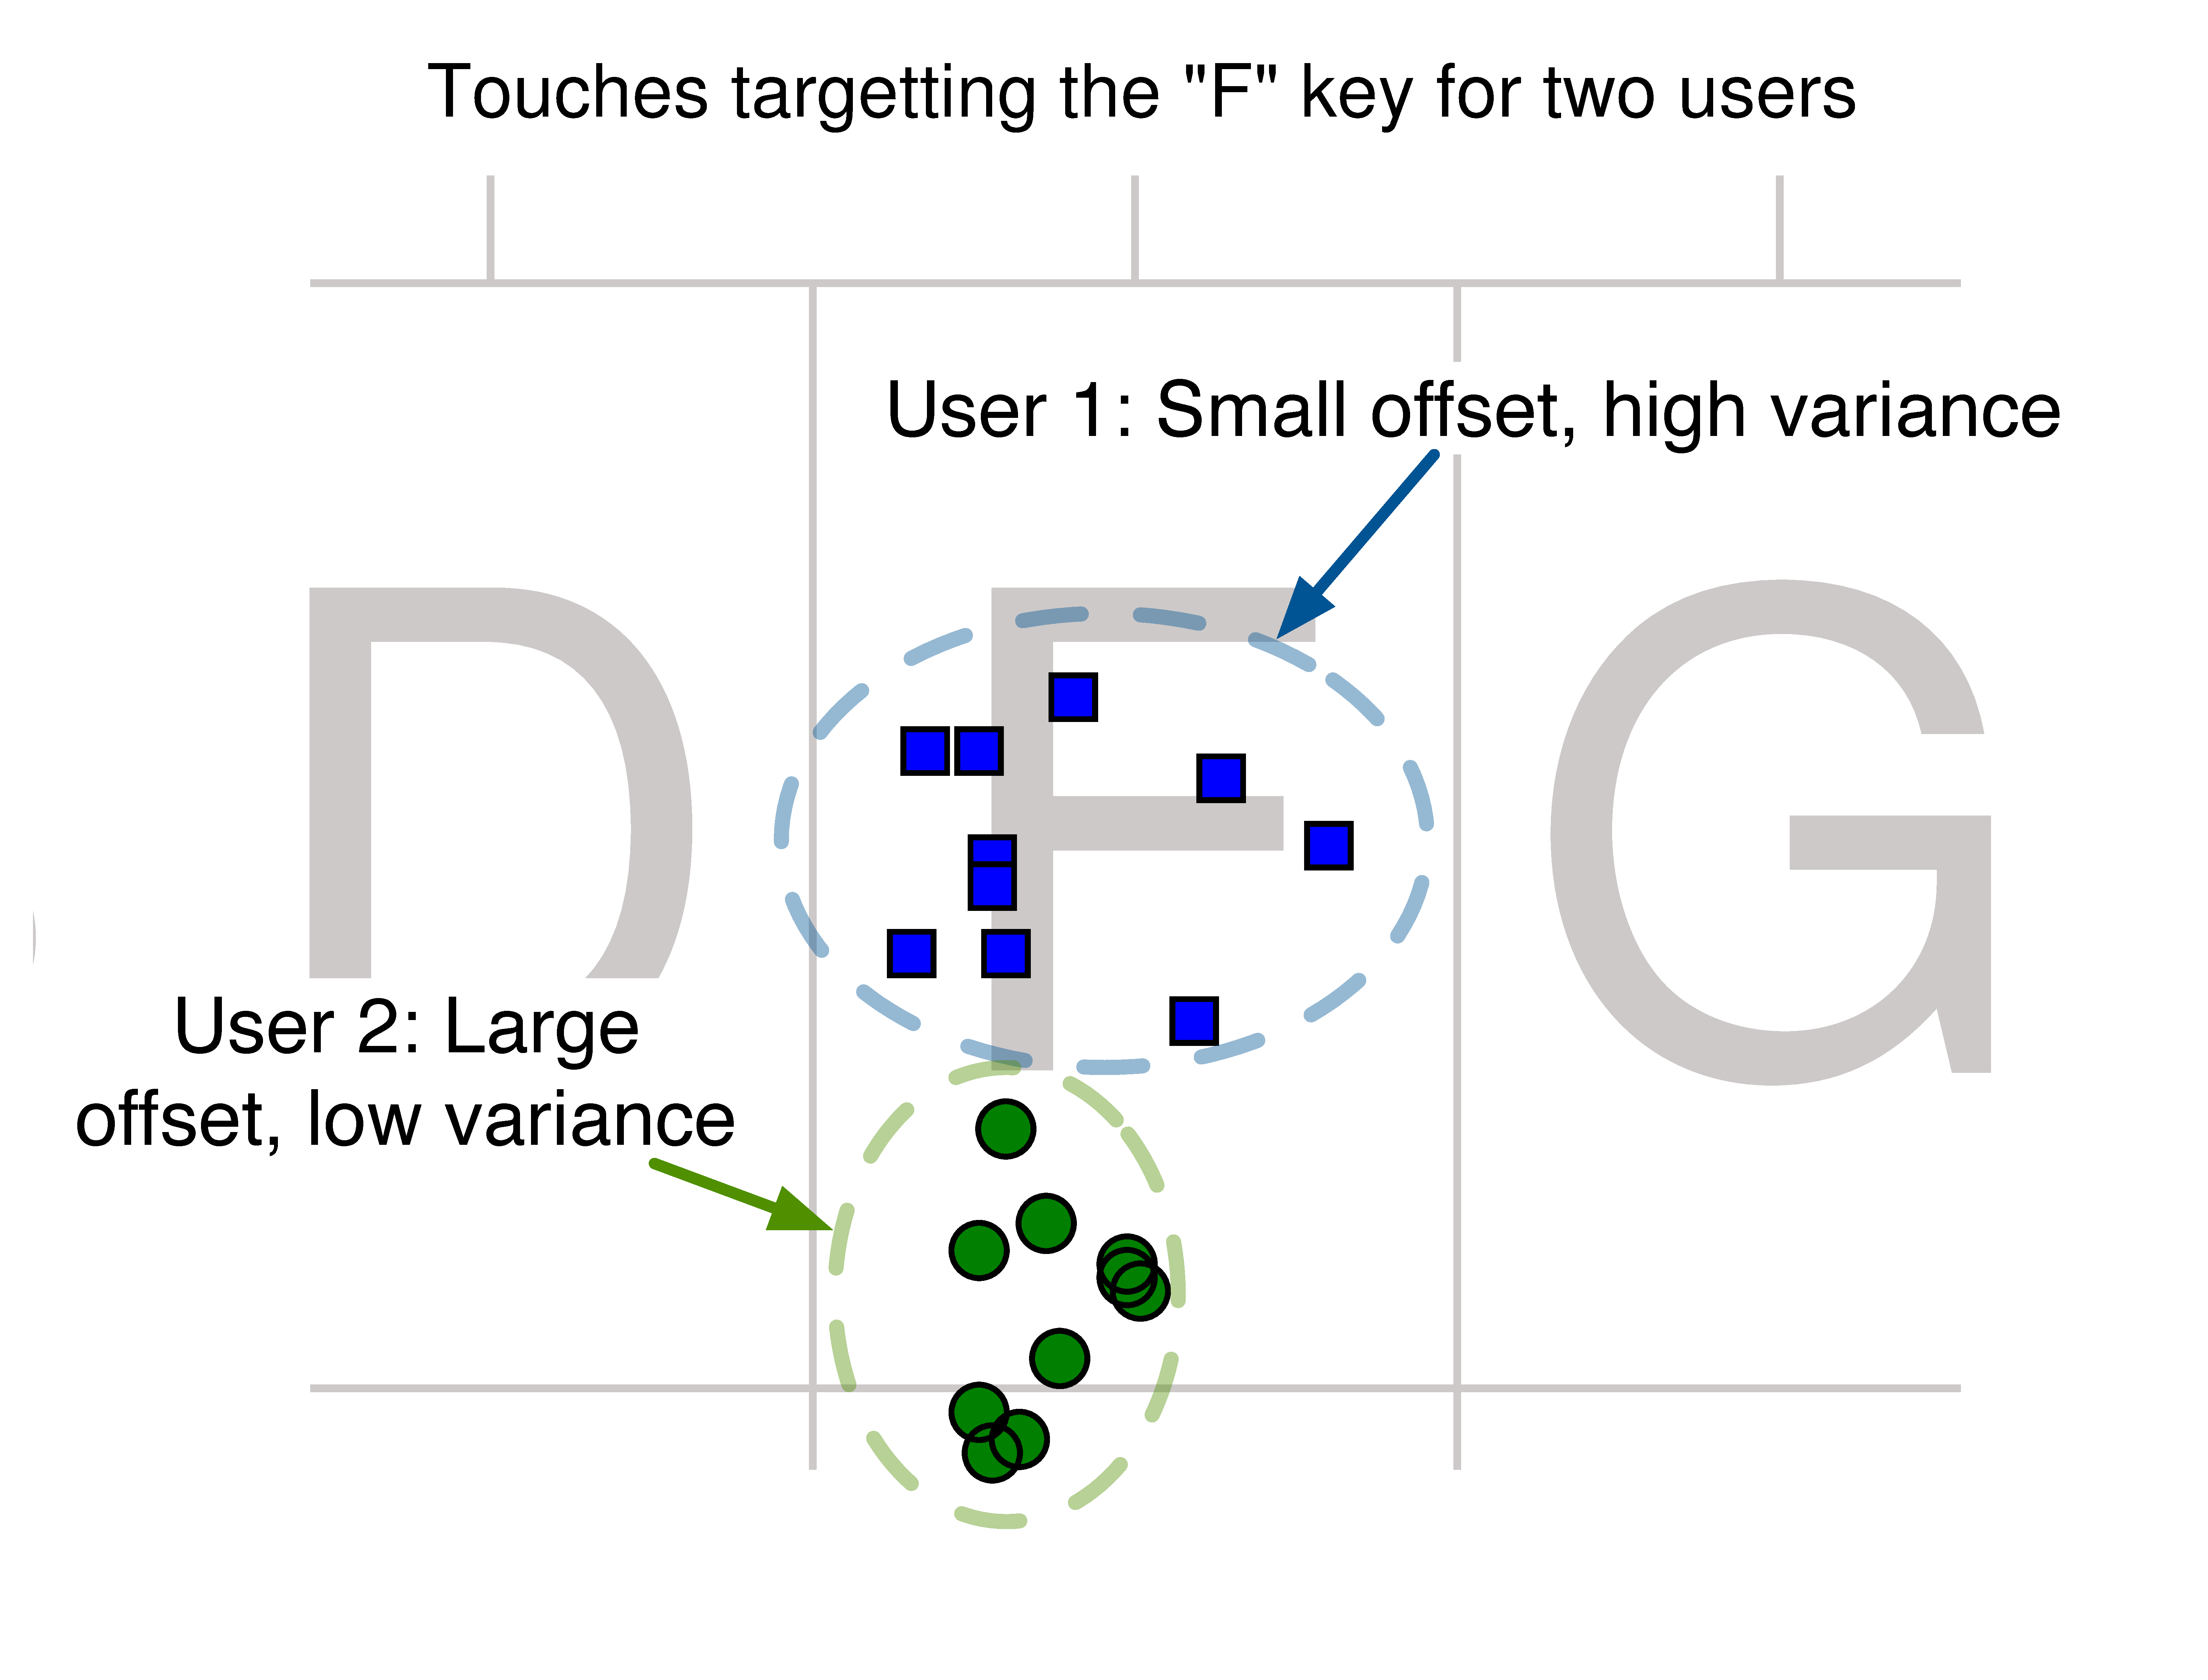
\includegraphics[width=0.8\linewidth]{two_users_annotated.pdf}
		\centering\caption{\label{fig:two_users_annotated}Touches recorded by two users aiming for the `F' key. User 2 has high bias and low variance, user 1 has low bias and high variance.}
	\end{figure}
\end{frame}

\begin{frame}
	\frametitle{Background 3: Current systems (maybe?)}
	\begin{itemize}
		\item Touch is boxed into nearest key.
		\item Key ID is passed to a \ac{SLM}.
		\item \ac{SLM} is made up of probabilities of observing certain character strings (from large text corpora).
		\item \ac{SLM} can swap characters to make the character string more likely.
		\begin{itemize}
			\item e.g. `HELLP $\rightarrow$ HELLO'
		\end{itemize}
	\end{itemize}
\end{frame}


\begin{frame}
	\frametitle{Our idea}
	\begin{itemize}
		\item There is a lot of uncertainty present in touch (bias and variance)
		\item Boxing a touch into a key is probably bad
		\item Why can't we pass a \emph{distribution} to the \ac{SLM}?
		\begin{itemize}
			\item Pass the uncertainty onwards
			\item Being Bayesian!
		\end{itemize}
		\visible<2->{
			\item Can use a user specific GP regression model to predict target from input touch.
		}
	\end{itemize}
\end{frame}

\begin{frame}
	\frametitle{The model}
	\begin{itemize}
		\item We use independent GP regressions for predicting $x$ and $y$ offsets.
		\item Training data:
		\begin{itemize}
			\item Each user typed phrases provided to them.
			\item Data: the $x,y$ location of the recorded touch (i.e. $\bx_n = [x_n,y_n]^T$). Target: the center of the intended key minus the touch (i.e. the offset).
		\end{itemize}
		\item<2-> Used a \ac{GP} with zero mean and a composite covariance:
		\[
			C(\bx_1,\bx_2) = a \bx_1^T\bx_2 + (1-a)\exp \{ -\gamma || \bx_1 - \bx_2 ||^2 \}
		\]
	\end{itemize}
\end{frame}

\begin{frame}
	\frametitle{The model}
	\centering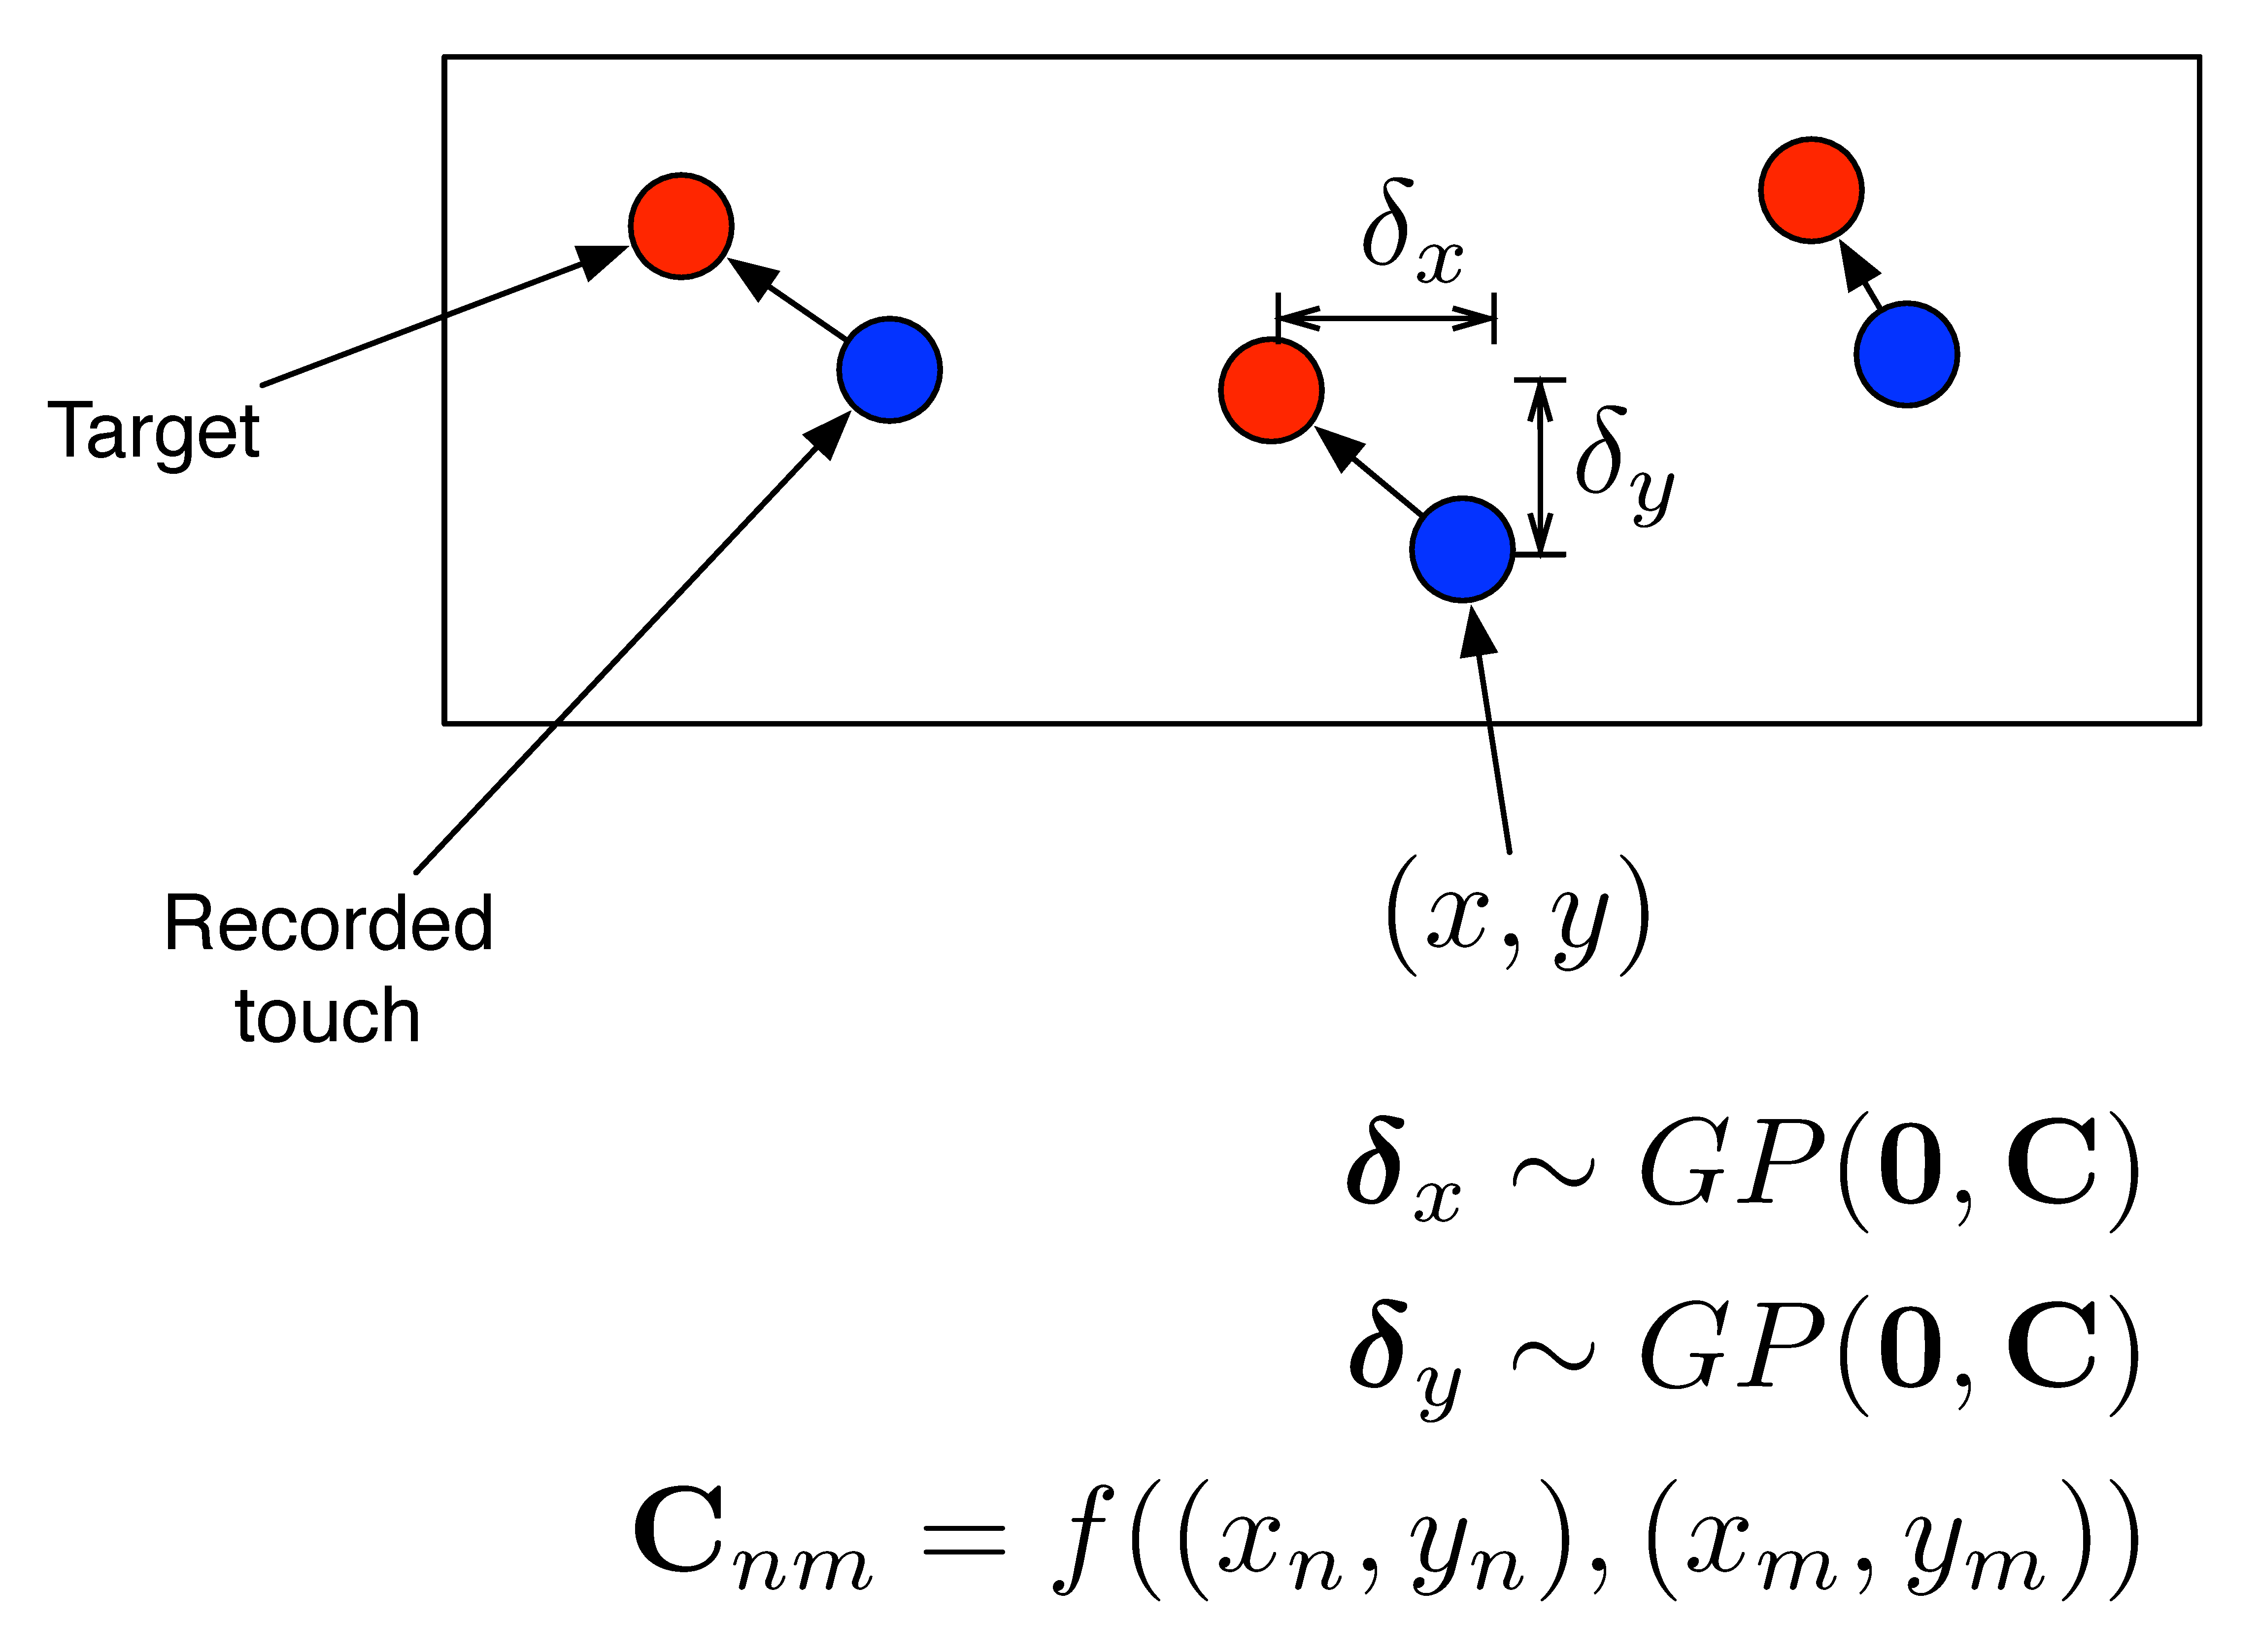
\includegraphics[width=0.7\linewidth]{touchmodel}
	\begin{itemize}
		\item $x$ and $y$ offsets both depend on $x$ and $y$ position of touch
		\item Have also used raw capacitive sensor data as input
		\begin{itemize}
			\item Potentially better (more info) but only accessible on some devices
		\end{itemize}
	\end{itemize}
\end{frame}


\begin{frame}
	\frametitle{System cartoon}
	\begin{figure}
		\centering\includegraphics<1>[width=0.8\linewidth]{cartoon1.pdf}
		\centering\includegraphics<2>[width=0.8\linewidth]{cartoon2.pdf}
		\centering\includegraphics<3>[width=0.8\linewidth]{cartoon3.pdf}
		\centering\includegraphics<4>[width=0.8\linewidth]{cartoon4.pdf}
		\centering\caption{Train GPs to predict the intended touch from an input touch. The flexibility of GPs means that the mean and covariance of the offset can vary across the keyboard.}
	\end{figure}
\end{frame}

\begin{frame}
	\frametitle{System cartoon}
	\begin{figure}[tbh]
		\centering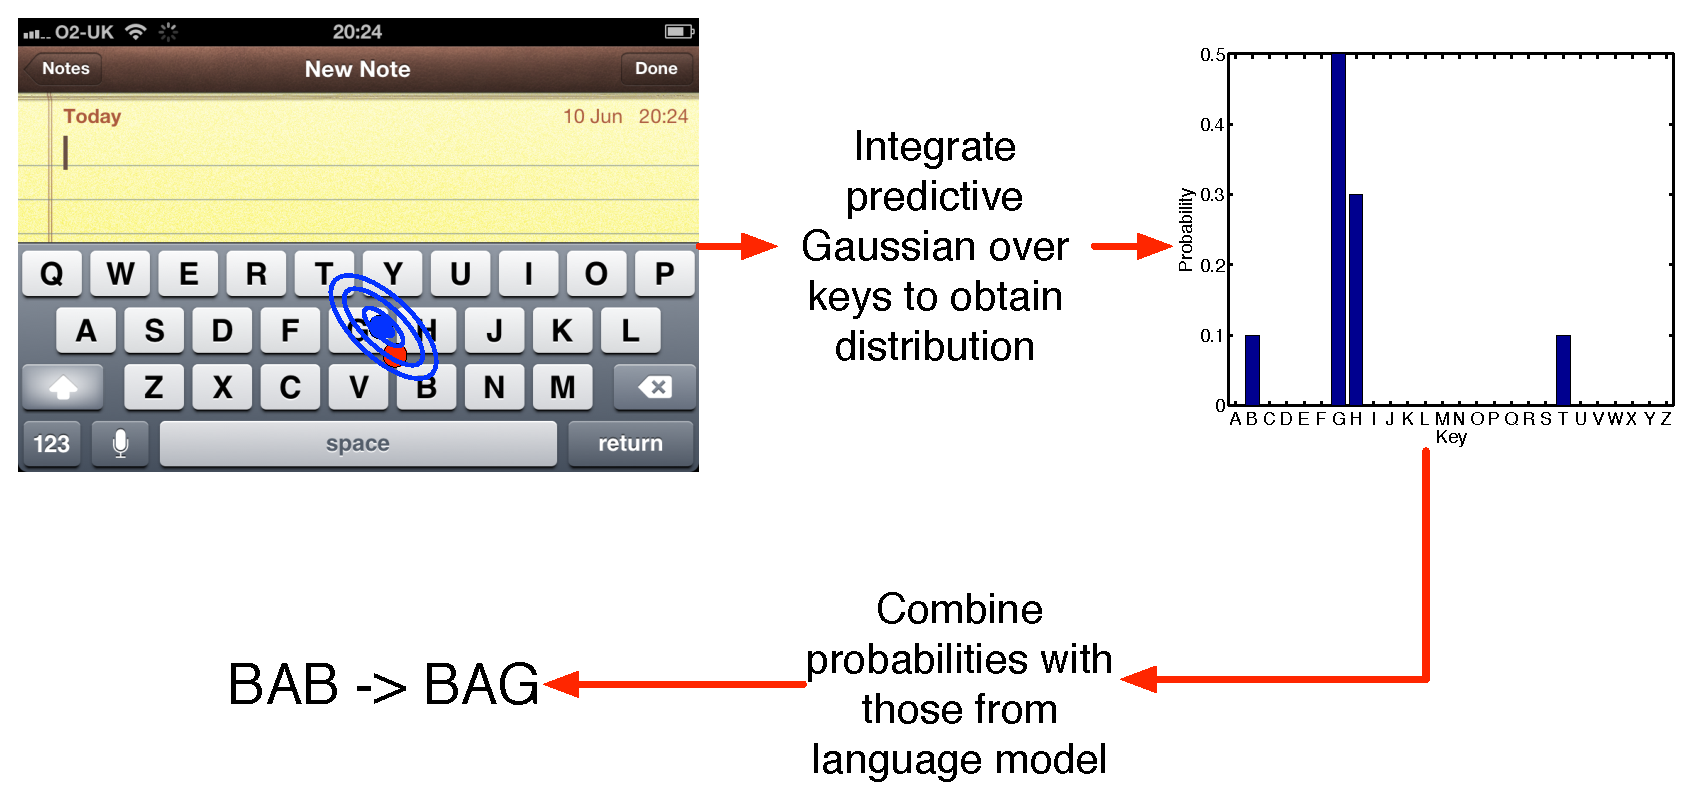
\includegraphics[width=\linewidth]{touchcartoon.pdf}
		\centering\caption{\label{fig:touchcartoon}The complete system}
	\end{figure}
\end{frame}


\begin{frame}
	\frametitle{Video}
	\begin{itemize}
		\item \url{http://www.youtube.com/watch?v=llQI5gV5l74}
	\end{itemize}
\end{frame}

\begin{frame}
	\frametitle{The experiment}
	\begin{itemize}
		\item 10 participants
		\item Calibration data collected for each
		\begin{itemize}
			\item Note: calibration task matters
		\end{itemize}
		\item each did $3\times$ 45 minute sessions, typing whilst sitting, standing and walking. [more details in paper]
		\item Compared:
		\begin{itemize}
			\item GPtype (our system), Swiftkey (commercial Android keyboard), GP only (just offset, no \ac{SLM}), baseline (boxing, no \ac{SLM}).
		\end{itemize}
	\end{itemize}
\end{frame}

\begin{frame}
	\frametitle{Results}
	\begin{figure}[tbh]
		\centering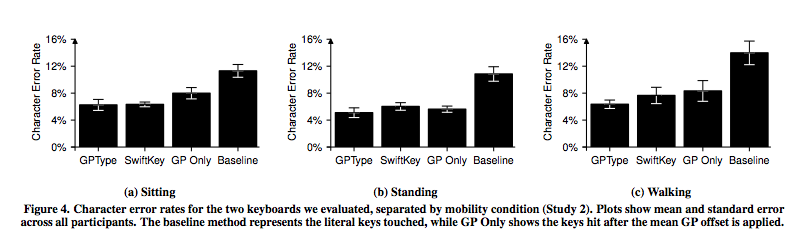
\includegraphics[width=1.0\linewidth]{gptype_results.png}
		\centering\caption{\label{fig:gptype_results}Results of GPType experiment}
	\end{figure}
	\begin{itemize}
		\item GPType marginally (stat sig) better than Swiftkey.
		\begin{itemize}
			\item A {\bf lot} of people work on SwiftKey
		\end{itemize}
		\item Baseline awful!
	\end{itemize}
\end{frame}

\begin{frame}
	\frametitle{Explicit uncertainity control}
	\begin{itemize}
		\item In GPType, uncertainity is handled implicitly
		\item As user typing becomes more uncertain, more power given to language model
		\item Could users \emph{explicitly} control this?
		\begin{itemize}
			\item Certain inputs: no \ac{SLM} control (slang, names, etc)
			\item Uncertain inputs: high \ac{SLM} control
		\end{itemize}
		\item Use pressure to control certainty:
		\begin{itemize}
			\item High pressure: high certainty
			\item Low pressure: low certainty
		\end{itemize}
	\end{itemize}
\end{frame}

\begin{frame}
	\frametitle{Do users know when \ac{SLM} will fail?}
	\centering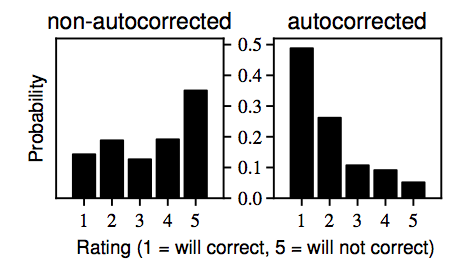
\includegraphics[width=\linewidth]{autocorrect}
	\begin{itemize}
		\item Users given phrases and asked whether they thought autocorrect would change them incorrectly
		\item Users quite good at understanding \ac{SLM} failings
	\end{itemize}
\end{frame}

\begin{frame}
	\frametitle{ForceType}
	\centering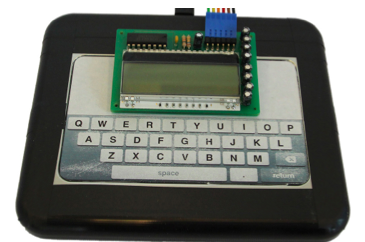
\includegraphics[width=0.6\linewidth]{forcetype}
	\begin{itemize}
		\item Modified Synaptics Forcepad
		\item Pressure mapped to Gaussian variance (no \ac{GP})
		\item System explained to users
		\item Users type phrases with and without forcetype
	\end{itemize}
\end{frame}

\begin{frame}
	\frametitle{ForceType: Results}
	\begin{multicols}{2}
		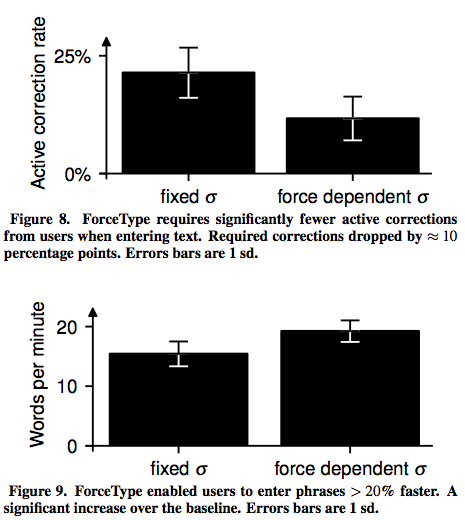
\includegraphics[width=\linewidth]{forcetype_results}
		\newpage
		\vfill
		\begin{itemize}
			\item Forcetype reduced number of corrections performed by users (top)
			\item Forcetype improved overall text entry rate
		\end{itemize}
		\vfill
	\end{multicols}
\end{frame}

\begin{frame}
	\frametitle{Conclusions}
		\begin{itemize}
			\item GP regression is key to the approach: we make no parametric assumptions (what would they be?)
			\item \ldots and get probabilistic predictions
			\item \ldots that can be fed to the \ac{SLM} -- (un)certainity is passed to the \ac{SLM}
			\item Performance is promising
			\item<2->Can also use pressure to provide explicit uncertainty control
			\item<3->More info:
			\begin{itemize}
				\item \url{http://www.youtube.com/watch?v=llQI5gV5l74}
				\item \url{http://pokristensson.com/pubs/WeirEtAlCHI2014.pdf}
				\item Acknowledgements: Daryl Weir, Per Ola Kristensson, Keith Vertanen, Henning Pohl
			\end{itemize}
		\end{itemize}
\end{frame}

